\subsection{Base-Policy Skill Learning and Retention}\label{sec:skill_retention}
These measurements concern dense-reward training of simple CDPR skills and their consolidation into a base policy, before full-task composition. Each skill uses the instruction and reset protocol in Section~\ref{sec:skill_acquisition}; placement tests start with the object already held. Learning a new skill can degrade previously learned behavior, although the same policy must retain all component skills to execute the complete multi-stage task.

\begin{figure*}[!t]
\centering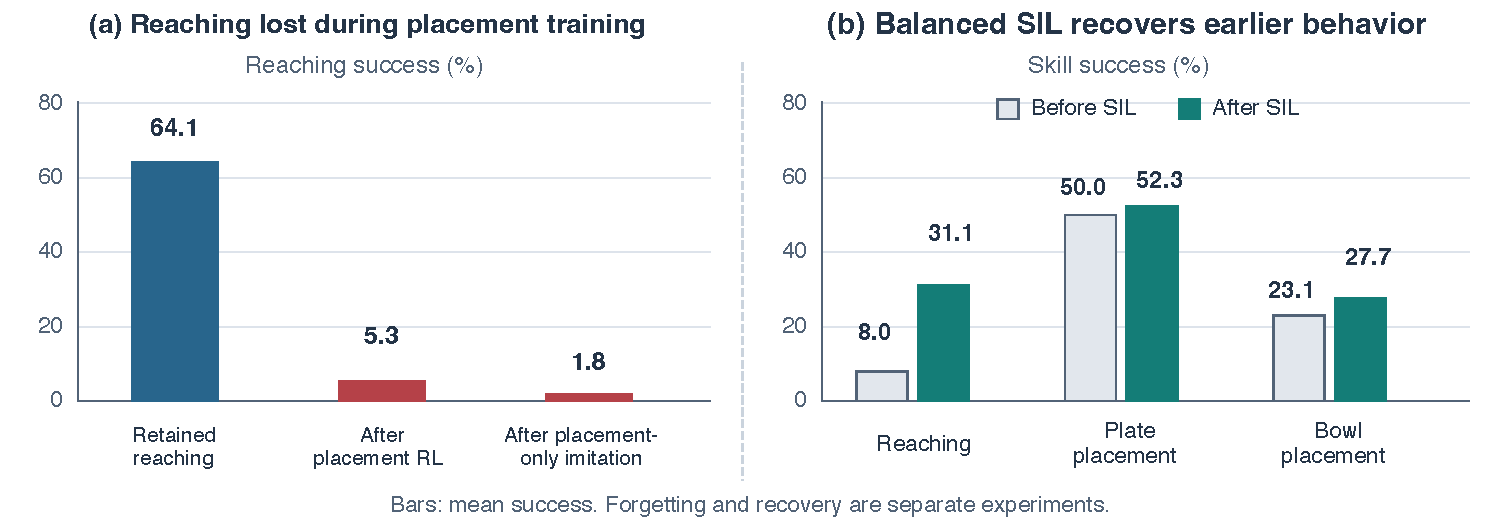
\includegraphics[width=\textwidth]{figures/skill_retention.pdf}
\caption{Base-policy skill recovery before full-task composition. Bars show means and points show individual evaluation rounds: three for reaching and two for each placement skill, per condition. Reaching uses the instruction \emph{move to \textless object\textgreater}; placement starts with the object already held. Reaching partially recovers while both placement means increase.}
\label{fig:retention}
\end{figure*}

In a forgetting evaluation, mean reaching success falls from 64.1\% for the reaching reference to 5.3\% after placement RL, over three evaluation rounds per condition. The recovery evaluation in Fig.~\ref{fig:retention} is a separate measurement: balanced self-imitation raises reaching success from 8.0\% to 31.1\%. Plate placement changes from 50.0\% to 52.3\%, and bowl placement from 23.05\% to 27.65\%. The bank combines earlier reaching successes with current placement successes, balancing the retained data by instruction.

Recovery is partial, with placement performance retained while reaching improves. Table~\ref{tab:skill_matrix} summarizes skill-specific RL references and a shared policy after subsequent consolidation. Evaluation reset distributions differ across stages. The shared policy succeeds on all four skills, although pickup remains weak. These skill evaluations do not isolate the contribution of self-imitation to final full-task success.

% Reaching reference: evidence/skill_retention_rounds.json, forgetting comparison.
% Other rows: ../CDPR_CONSOLIDATED_PROGRESS_REPORT.md, instruction success table;
% consolidation is the Cycle 3 shared policy, evaluated before composition.
\begin{table}[!ht]
\caption{Skill success (\%) by training stage. Placement starts with the object held; --- denotes an unreported result.}
\label{tab:skill_matrix}\centering\small
\begin{tabular}{@{}lrrrr@{}}\toprule
Training stage & Reach & Pickup & Plate & Bowl\\\midrule
Reaching RL & 64.1 & --- & --- & ---\\
Pickup RL & --- & 26.0 & --- & ---\\
Placement RL & --- & --- & 71.0 & 32.0\\
After consolidation & 47.8 & 11.9 & 73.8 & 53.5\\\bottomrule
\end{tabular}
\end{table}

